\documentclass[a4paper,notitlepage,parskip=half]{scrartcl}

\usepackage{color}
\usepackage{ngerman}
\usepackage{graphicx}
\areaset[1cm]{16cm}{26cm}
\usepackage{float}
\usepackage{fancybox}
\usepackage[T1]{fontenc}
\usepackage[utf8]{inputenc}
\usepackage{pifont}
\usepackage{url}
\usepackage{booktabs}
\usepackage{amsmath}
\usepackage{listings}
\usepackage[german]{varioref}
\usepackage{colortbl} % Farbige Tabellen
\usepackage{tabularx} % Mehrzeilige Tabellenzellen (nicht benutzt)
\usepackage{longtable}
%\usepackage[german,scrtime,time]{prelim2e}
%\usepackage{svn}
\usepackage{marginnote}
\usepackage{xcolor}
\graphicspath{{./jpg/}}
\DeclareGraphicsExtensions{.jpg,.eps,.png}
%\usepackage{courier}

\usepackage[most]{tcolorbox}
\usepackage{tikz}
\usetikzlibrary{intersections}
\usetikzlibrary{
  arrows,
  decorations.pathreplacing,
  shapes.symbols
}

% Wenn pdflatex benutzt wird sollen die 
% installierten! frutiger-Fonts verwendet werden
% Ansonsten cmbright
\ifpdfoutput %
{%
\usepackage[scaled=0.90]{frutiger}
\renewcommand\familydefault{\sfdefault}
%\DeclareFixedFont\ott{T1}{phv}{mc}{n}{10pt
}%
{%
\usepackage{cmbright}
}%


% falls man das auch noch ändern möchte
\newcommand{\pihk}{PIHK\ }
\newcommand{\titel}{PIHK}
\newcommand{\vnr}{3.0.0}

%\newcommand{\ffile}[1]{\par\centerline{\tt#1}\par}
\newcommand{\ffile}[1]{{\texttt{#1}}}
\newcommand{\cfile}[1]{{\texttt{#1}}}
\newcommand{\ttctable}[1]{\centerline{\texttt{#1}}}
\newcommand{\sname}[1]{\emph{#1}}
\definecolor{listinggray}{gray}{0.95}
\definecolor{OliveGreen}{rgb}{0,0.5,0}
\definecolor{pastellblau}{rgb}{0.85,0.95,1.0} 

\newcolumntype{g}{>{\columncolor{pastellblau}}l}

\lstset{numbers=left,numbersep=5pt,numberstyle=\tiny,%
    frame=none,basicstyle=\scriptsize\ttfamily,breaklines=true,%
    captionpos=b,backgroundcolor=\color{listinggray},frame=single}

% \parindent0cm
% \parskip1ex
\setlength{\parindent}{0em}

%\usepackage{courier}
\newtcolorbox{marker}[1][]{enhanced,
  before skip=2mm,after skip=3mm,
  boxrule=0.4pt,left=5mm,right=2mm,top=1mm,bottom=1mm,
  colback=yellow!50,
  colframe=yellow!20!black,
  sharp corners,rounded corners=southeast,arc is angular,arc=3mm,
  underlay={%
    \path[fill=tcbcolback!80!black] ([yshift=3mm]interior.south east)--++(-0.4,-0.1)--++(0.1,-0.2);
    \path[draw=tcbcolframe,shorten <=-0.05mm,shorten >=-0.05mm] ([yshift=3mm]interior.south east)--++(-0.4,-0.1)--++(0.1,-0.2);
    \path[fill=yellow!50!black,draw=none] (interior.south west) rectangle node[red!20!white]{\Huge\bfseries !} ([xshift=4mm]interior.north west);
    },
  drop fuzzy shadow,#1}


\begin{document}

\titlehead{\centerline{Frank Zimmermann \ding{70} Software \ding{70} Tools }}
% %\titlehead{\includegraphics{zenlogo}}
% \subject{Dokumentation}
%\title{PIHK \\[1.0ex] \small Letztes Änderungsdatum \SVNDate\\ geändert von \SVNLastChangedBy\\ DocRevision\SVNLastChangedRevision}
\title{PIHK\\{\small Version \vnr}}
\subtitle{Programm zur Unterstützung bei IHK--Prüfungen\\[2ex]{\small Letztes Änderungsdatum\\  \today} }
\author{Frank Zimmermann\\[1ex]{\small fz@zenmeister.de}}
\date{Erstellungsdatum: 20.06.2016}
\maketitle

\begin{abstract}
\setlength{\parindent}{0em}
Diese Dokumentation beschreibt das Programm \pihk in der Version \vnr.\\ 
\end{abstract}
\rule{\linewidth}{1pt}
\tableofcontents
\rule{\linewidth}{1pt}

\newpage


\section{Motivation}
Das Programm \pihk wurde geschrieben, um bei IHK--Prüfungen der Fachinformatiker
bei der IHK--Hannover eine Hilfe bei der Berechnung und Vergabe der Punkte zu sein. Dabei wurden die 
Regularien der IHK--Hannover zugrunde gelegt. Eine Verwendung bei anderen Prüfungen
ist natürlich möglich, sofern die Regularien zur Berechnung identisch sind.
Die genauen Regularien stammen aus dem Dokument:

\begin{quote}
\emph{Verordnung über die Berufsausbildung im Bereich der Informations-- und Telekommunikationstechnik  (veröffentlicht im Bundesgesetzblatt Teil I Nr. 9 vom 05. März 2020)}
\end{quote}



\section{Funktion des Programms}
Die erste Funktion des Programms ist die Berechnung der Punkte/Noten in den Teilen 1 und 2 der Prüfung und die Berechnung der Gesamtpunktzahl/Gesamtnote.

Dabei ist die Berechnung der Punkte gerade bei einer mündlichen Ergänzungsprüfung (MEPR) von großem Nutzen, da während einer Prüfung  das Berechnungsverfahren recht unübersichtlich ist.

Die zweite Funktion des Programms ist eine Simulation der Gesamtergebnisse und der Teilergebnisse in der Teilprüfung T21 (Präsentation und Fachgespräch )  und bei der Vergabe der Punkte in der MEPR (für T22,T23 oder T24).

Damit ist es leicht möglich, Notengrenzen zu erkennen und ggfs. Notengrenzen bei der Vergabe der Punkte zu beachten.

\section{Das Programm}

\begin{figure}[ht]
	\centering
  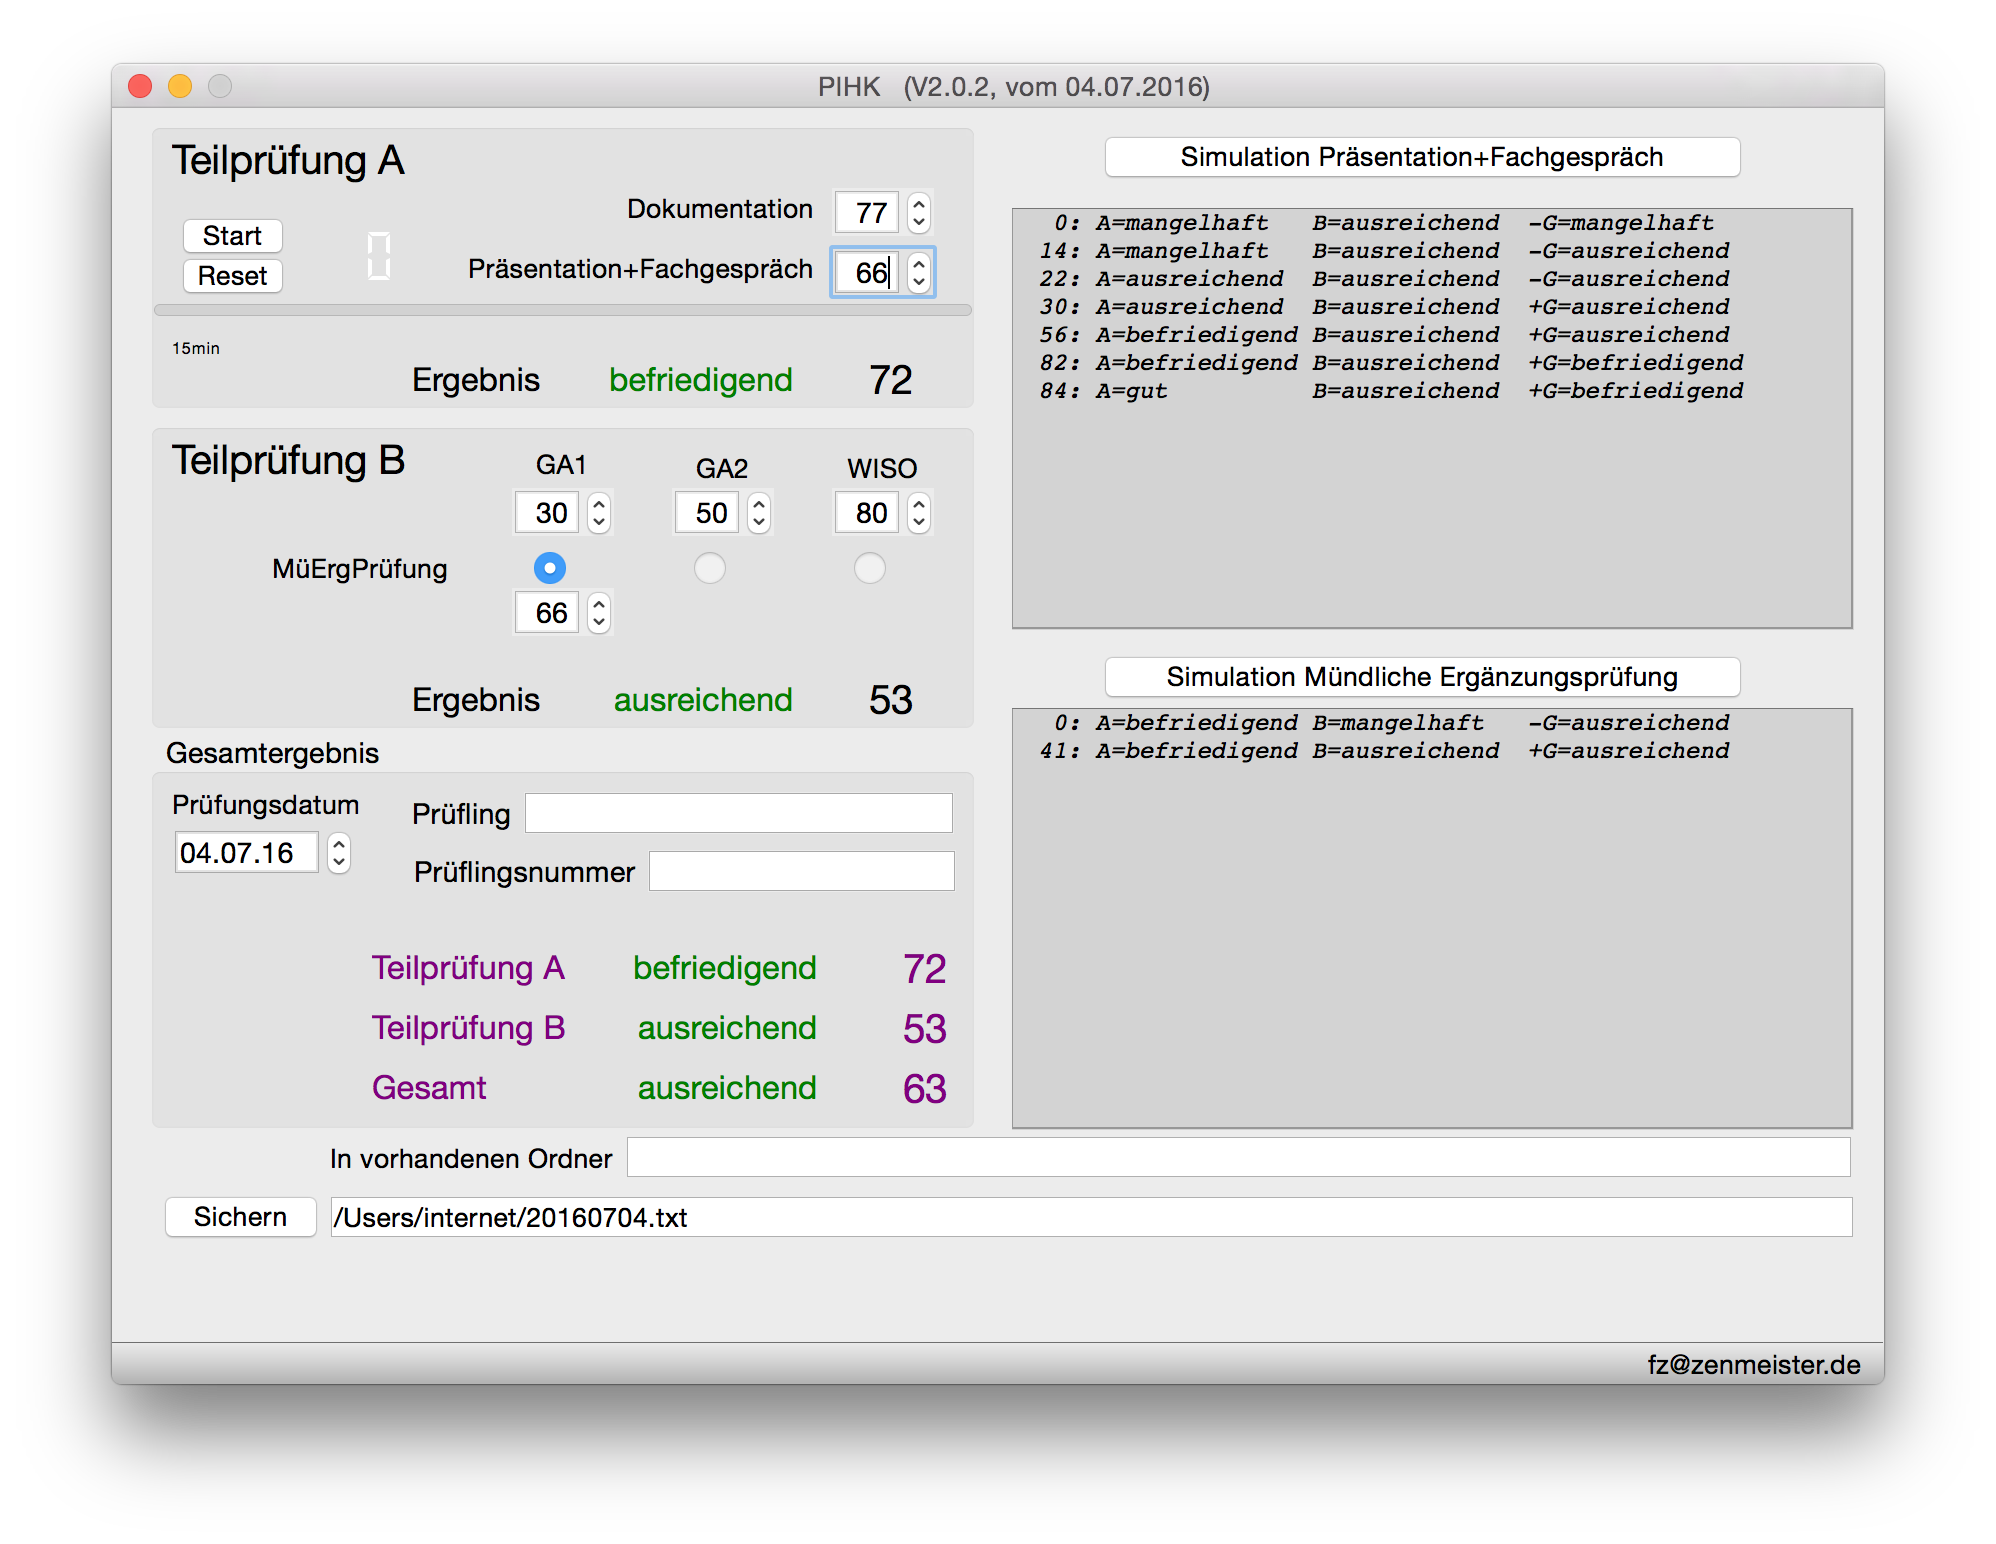
\includegraphics[width=\textwidth]{pihk.png}
	\caption{Programmoberfläche}
	\label{fig:pihk}
\end{figure}

Das Programm (siehe Abb.\ref{fig:pihk}) gliedert sich grob in 2 Bereiche, links und rechts:

Links ist der Bereich zur Eingabe und Berechnung der Punktzahlen und Noten.

In den oberen Bereich trägt man die Klausurergebnisse für den Teilbereich~1 ein, der mit 20 \% in die Gesamtnote eingeht.

\subsection{Prüfungsbereich Teil 1} 
Da die Präsentation während der Prüfung ca. 15 Minuten dauern soll, findet man oben auch eine kleine Stopp-Uhr, mit der man die tatsächlich gehaltene Vortragszeit messen kann.

Diese startet bei Drücken des \framebox{Start}--Buttons und wird durch Drücken des \framebox{Stop}--Buttons wieder gestoppt. 
Mit \framebox{Reset} setzt man alles wieder zurück.
Bei Unterbrechungen kann man die Uhr stoppen und wieder starten.
Bei Überschreitung der 15 Minuten wird neu hochgezählt (mit 1 beginnend) damit man sofort die Überziehungszeit ablesen kann.

Die 15 Minuten Prüfungszeit sind im Einstellungsdialog konfigurierbar (1..99 Minuten) und können mit dem Programm abgespeichert werden.

\subsection{Prüfungsbereich Teil 2}
Im nächsten linken Bereich können die Daten für den Prüfungsbereich 2 eingegeben werden.

\subsubsection{Prüfungsbereich T21}
Im Prüfungsbereich T21 wird eine Dokumentation (T21a) über ein durchgeführtes Projekt und eine Präsentation mit anschliessendem Fachgespräch (T21b) durchgeführt. Beide Teilprüfungen gehen mit gleichem Gewicht in das Ergebnis von T21 ein. Während das Ergebnis der Präsentation (T21a) in der Regel schon feststeht und einfach eingetragen werden kann, wird das Ergebnis der anderen Teilprüfung erst nach Beratung des Prüfungsausschusses am Prüfungstag ermittelt.
Die Note für den Prüfungsbereich T21 geht zur Ermittlung des Note im Teilbereich 2 ein (Gewichtung 25~\%) und bestimmt die Endnote mit einer Gewichtung von 50~\%.

Um die zu vergebenen Punkte in T21b nicht so ungünstig zu vergeben, dass eine Endnote womöglich nur um einen (oder rechnerisch sogar einen halben) Punkt unter der nächsten Notengrenze liegt, dient die im rechten Bereich durchgeführte Simulation für das Ergebnis des Teilbereichs T21b. 


\subsubsection{Prüfungsbereich T22,T23 und T24}

Links unten findet man Angaben zur Prüfung, wie Datum der Prüfung und Name und Nummer des Prüflings.
Die Angaben werden dabei benutzt um einen Dateinamen zu generieren, der unten angezeigt wird. Dabei erfolgt die Speicherung der Datei automatisch im \framebox{Home}--Verzeichnis des Benutzers.
Soll die Speicherung in einem schon existierenden Ordner erfolgen, so kann dieser auch angegeben werden; nur wenn dieser existiert wird der entsprechende Speicherpfad entsprechend korrigiert (dabei ist zu beachten, dass z.B. der Dokumenten--Ordner oft intern als Documents anzugeben ist).

Der \framebox{Sichern}--Button sichert die Datei mit allen erfassten Informationen unter dem aktuellen Namen und wird dann deaktiviert. Erst bei Änderungen wird dieser Button wieder aktiviert.

Rechts ist der Bereich zur Simulation der Punkte. 

Dabei wird rechts oben die Note für die Präsentation und das Fachgespräch simuliert. In einer Liste werden die Punkte aufgelistet, die eine Veränderung der Noten in den Teilbereichen und in der Gesamtbewertung zur Folge hätten.

Rechts unten wird die Punktzahl der mündlichen Ergänzungsprüfung (MEPR) in dem angewählten Prüfungsbereich zur MEPR simuliert. Die Liste gibt wieder die Punktzahlen der MEPR an, bei denen eine Veränderung der Noten in den Teilbereichen und der Gesamtbewertung erfolgt. 

\section{Rundung}
Bei der Berechnung der Punkte nach dem Formular, das bei der Prüfung benutzt wird, ist darauf zu achten, wann die errechneten Werte gerundet werden (betrifft nur Teilbereich B).

Ohne mündliche Ergänzungsprüfung werden nur ganze Zahlen als Punktwerte eingetragen und am Ende für die 3 Prüfbereiche berechnet;
hier erfolgt dann die einzige vorzunehmende Rundung des Ergebnisses.

Anders sieht es beim Vorhandensein einer mündlichen Ergänzunmgsprüfung aus. Diese geht mit ihrer ganzzahligen Punktzahl nur zu einem Drittel in die Punktzahl des Prüfbereichs ein. Das Ergebnis für diesen Prüfbereich ergibt sich daher durch eine Division und müsste
in das IHK--Prüfungsformular eingetragen werden. Hierbei soll eine Rundung auf einen ganzahligen Wert erfolgen. Die weitere Rechnung ergibt dann wieder den Wert für alle Prüfbereiche und muss muss daher ebenfalls gerundet werden.

Bei einer korrekten 2-maligen Rundung wird also zum ersten mal bei der Berechnung des nachgeprüften Prüfbereiches inklusive der mündlichen Ergänzungsprüfung gerundet und das zweite mal bei der Berechnung aller Prüfungsbereiche.
\vskip2ex

\fcolorbox{black}{listinggray}{\parbox{\linewidth}{%
\vskip1ex
Gegeben seien beispielsweise folgende Punkte im Teilbereich B:
\begin{center}GA1=30,  GA2=49,  WISO=82, MEPR in GA2E= 60\end{center}
Mit \emph{einer} Rundung ergäbe sich als Note für Teilbereich B =49 Punkte und damit mangelhaft:
$$Round( ( ((GA2*2+MEPR)/3) * 2 + GA1 * 2 + WISO)/5)$$
$$Round( ( ((49*2+60)/3) * 2 + 30*2+82)/5)=49,47=49$$
Mit \emph{zwei} Rundungen ergibt sich als Note für den Teilbereich B =50 Punkte und damit ausreichend:
$$Round( ( Round((GA2*2+MEPR)/3)*2+GA1*2+WISO)/5) $$
$$Round( ( Round((49*2+60)/3) * 2 + 30*2+82 )/5)=49,6=50$$

}}
\vskip2ex

Das zeigt, dass es für den Prüfling  manchmal sehr entscheidend ist, wann und wo gerundet wird!

Die doppelte Rundung ist aus dem \emph{Prüfungskompass, IHK--Hannover (Handbuch zum Prüfungswesen~1,2014,S.147, ISBN:978-3-942951-13-5)} entnommen.

Das Programm führt nach dieser Empfehlung daher zwei Rundungen aus.

\section{Benutzung}
Das Programm erfordert keine Installation und kann von jedem Ort gestartet werden.

Ein empfohlener Arbeitsfluss (kann ansonsten beliebig sein):

\begin{enumerate}
\item Prüfungsdatum eintragen
\item Prüfling (und bei Zweideutigkeiten ggfs. Nummer) eintragen
\item (Optional) Eigenen Ordner eintragen
\item Dokumentation, GA1,GA2,Wiso eintragen
\item Nach Fachgespräch (unter Berücksichtigung der Simulation) die Punkte eintragen
\item Bei MEPR: Prüfungsbereich anwählen und (Simulation!) Punkte eintragen
\end{enumerate}

Wird eine Zeile in der Simulation (PRFG oder MEPR) angeklickt, so werden die entsprechenden Punkte in die linke
Maske eingetragen.

\section{Ausgabe}
Die Datei, die gespeichert wird hat folgenden Inhalt:
\nopagebreak[4]

\begin{minipage}[t]{\textwidth}
\begin{lstlisting}[numbers=none,caption={\cfile{Gesicherte Datei: $20160621Max\_Mustermann13145678.txt$}},label=lst:datei]
Datum     : 21.06.16
Name      : Max Mustermann
Id-Nummer : 13145678
Doku      : 77
PRFG      : 66
GA1       : 30
GA2       : 50
Wiso      : 80
MEP-GA1   : 66
MEP-GA2   : 0
MEP-WISO  : 0
Ergebnis A:  72 (befriedigend)
Ergebnis B:  53 ( ausreichend)
Ergebnis  :  63 ( ausreichend)

---BESTANDEN---
\end{lstlisting}
\end{minipage}
Leerzeichen im Prüfungsnamen werden automagisch zu einem Unterstrich ($\_$) konvertiert, um Probleme mit dem Betriebssystem zu vermeiden.

\section{Plattform}
Das Programm wurde sowohl für Microsoft Windows als auch für Apple OSX programmiert und steht für beide Plattformen zur Verfügung.

Getestet und entwickelt wurde für MS Windows auf Win~10 und für Apple~OSX auf Yosemite(10.10.x).

Es wird für MS~Windows als \texttt{.exe} und für Apple~OSX als \texttt{.dmg} Datei zur Verfügung gestellt. 

\section{Programmpflege}
Das Programm wurde ohne finanzielles Interesse zur Erleichterung der eigenen Arbeit erstellt.
Das Programm kann von anderen frei genutzt werden, eine Verantwortung zur Pflege des Programms erwächst dem Autor deshalb nicht.

Sollten dem Autor Fehler gemeldet werden, so werden diese \emph{nach Möglichkeit} korrigiert. Hinweise und Fehler sollten per Email an die hier angegebene Adresse gesandt werden.

Das Programm wurde erstellt von:

Frank Zimmermann\\
fz@zenmeister.de

Es sei darauf hingewiesen, dass die IHK--Hannover keinerlei Verantwortlichkeiten für dieses Programm besitzt.
\section{Änderungshistorie}
\begin{table}[H]\centering
\begin{tabular}{|l|l|r|}
\hline
Datum & Änderung &Version\\
\hline
x.11.2021&	Anpassung an neue Prüfungsordnung	&  3.0.0\\
11.2.2020&	Windows Version						&  2.2.0\\
4.7.2016&	Initiale, ungetestete Version		&  2.1.0\\
23.6.2016&	XPlattform-Version, doppelte Rundung&  2.0.1\\
04.7.2016&	Klick in Simulation trägt Punkte ein&  2.0.2\\
\hline
\end{tabular}
\caption{Änderungshistorie}
\end{table}

\begin{marker}
In der heutigen Zeit verlangen viele Platformen eine relativ teure Registrierung für Entwickler, damit die Programme leicht auf den Platformen installiert werden können. Erfolgt keine Signierung und Authentfizierung melden die Platformen i.a. gefährlichen Code. 
\end{marker}

\end{document}